\chapter{Auto-scaling Techniques}
\label{intro-auto-scale}

As mentioned in Chapter~\ref{prob-def} the key characteristic of cloud environments is \emph{elasticity} behavior. However, manually adjusting resources are is not an effective approach to exploit this feature. Hence, we need to automate this procedure with minimal human intervention. This chapter introduces foundations of Auto-Scaling techniques. Different techniques and architectures will be discussed from a high level standing point. A detailed introduction into the topic is given by~\textcite{Lorido-Botran2014}. This chapter is organized as follows. Section~\ref{ias:basics} introduces basic concepts of Auto-Scaling. Section~\ref{ias:arch} defines general architecture of an Auto-Scaler. Section~\ref{ias:actions} clarifies which sort of actions can be applied by an Auto-Scaler. Section~\ref{ias:taxonomy} classifies different techniques and briefly explains each category. Finally, Section~\ref{ias:conc} concludes.

\section{Basic Concepts}
\label{ias:basics}

The ultimate goal of an Auto-Scaling system is to automate the process of acquiring and releasing \emph{resources} in order to minimize the \emph{cost} with minimum violation of \emph{service level objectives} (SLO). However, \emph{resource} is a broad and context-dependent term. It refers to any form processing unit -- engine -- that provides application developers some form of computation power. This general purpose definition is broad enough to capture different kinds. In most cases, it means virtual machines allocated by cloud provider. In more modern distributed systems, it may refer to \emph{container}s like Docker Container Engine~\cite{docker}. However, a resource might be as simple as a single process or thread.

The term \emph{cost} refers to any form of expenditure that users pay in order to acquire a resource. It doesn't necessarily mean \emph{monetary} cost. It can also refer to numerical values of resources, like number of virtual machines or number of running processes. Although minimizing cost is the ultimate goal of any Auto-Scaling system, not in all cases cost reduction is desirable. It should be achieved with respect to defined \emph{Service Level Objectives} (SLO).

\emph{Service Level Objectives} are any predefined rules that shall be respected during application runtime. The following defines a couple of SLOs for different applications:
\begin{itemize}
    \item 99 percentile round-trip latency of requests in a web application should be less than 150 milliseconds.
    \item All committed records in master database must be replicated with a maximum delay of 5 milliseconds.
    \item All messages pushed by a producer, should be processed by respective consumers in less than 5 minutes.
    \item At least 95\% of images published in the last 24 hours should be served by cache servers.
\end{itemize}
Defining effective and meaningful SLOs is a challenge on its own. Typically, it requires coordination with business team. Having profound understanding of system requirements is critical to define appropriate SLOs~\cite{Walter:2017}. However, it is out of the scope of this thesis. In this thesis, it is assumed that there is a well established set of pre-defined SLOs.

From a high level point of view, Auto-Scaling is a \emph{trade-off} amongst cost and violation of SLOs. Resource \emph{under-provisioning} will degrade performance and leads to SLO violations, while on the other hand, resource \emph{over-provisioning} leads to idle resources, hence unnecessary costs. To make an effective decision, an Auto-Scaler needs to consider application and its environment:
\begin{itemize}
    \item \textbf{Infrastructure pricing model}. Some infrastructure providers charge customers on hourly basis. That is, if customer acquires a resource at 10:30AM and releases it at 11:30AM, the customer is charged for two hours. Some other service providers might charge on minute basis. Pricing model has a huge impact on aggressiveness of the Auto-Scaler system, since it makes some decisions pointless.
    \item \textbf{Service level objectives}. Each application has its own set of objectives that should be adhered by Auto-Scaling system. These SLOs might be defined and applied at \emph{soft} and \emph{hard} levels. Violating an SLO at soft level is not critical, albeit alarming. However, violating a resource at hard level is a critical issue and is a negative point for an Auto-Scaler.
    \item \textbf{Acquire/Release delay}. Depending on type of the resource, it might take some time for the resource to become responsive and ready to process user requests. For example, booting a virtual machine typically takes couple of minutes, whereas launching a container takes time in order of seconds. An Auto-Scaler shall consider whether acquiring and releasing a heavy weight resource in a \emph{zig-zag} manner worth the overhead or not.
    \item \textbf{Unit of allocation}. In some cases, it might be beneficial to allocate multiple instances of a same resource at once. This might be due to the startup and initialization overhead or it might be the case that Auto-Scaler predicted a huge load spike in near future.
\end{itemize}

\section{Generic Auto-Scaler Architecture}
\label{ias:arch}
Figure~\ref{fig:auto-scaler-arch} illustrates generic architecture of an Auto-Scaler. This architecture is broad enough to capture different kinds of applications.
\begin{figure}[!htbp]
    \centering
    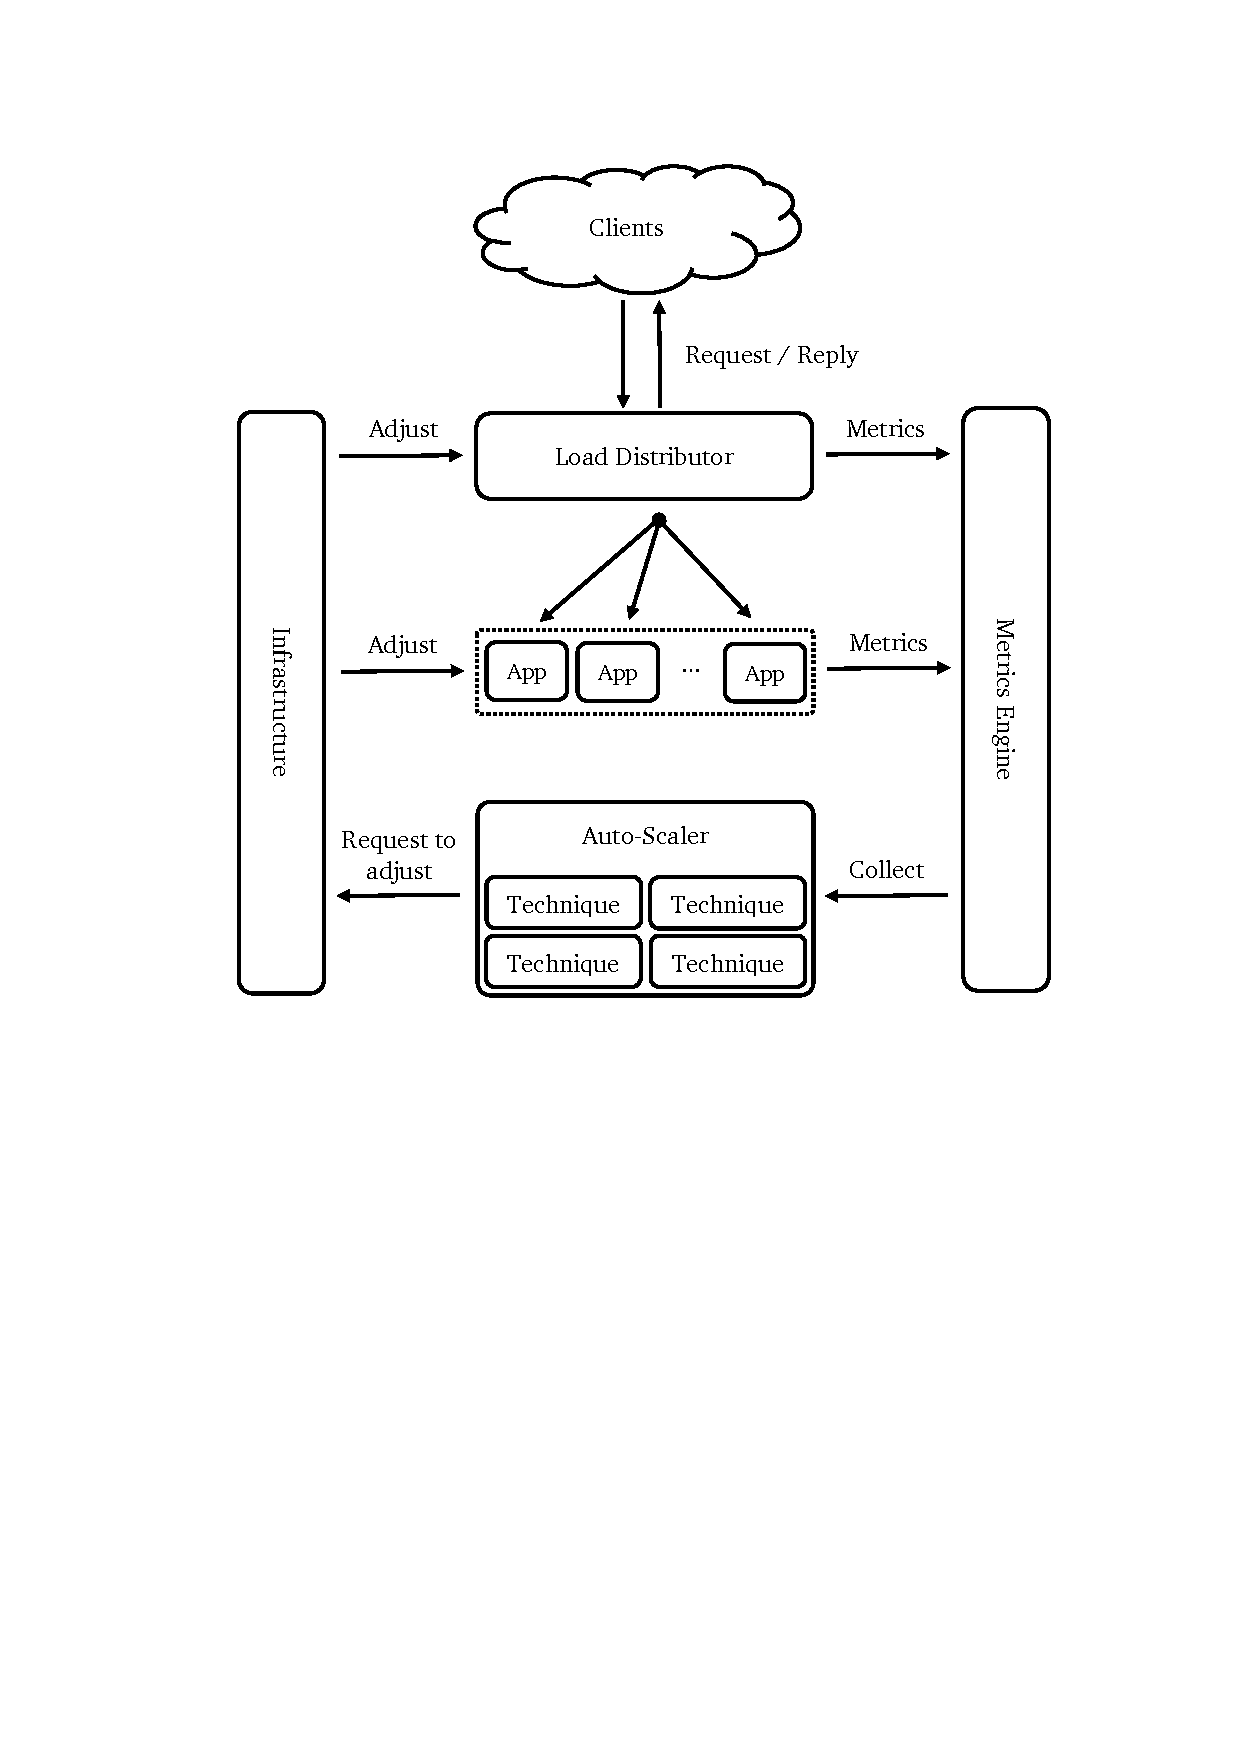
\includegraphics[clip, trim=3cm 12.5cm 2.5cm 2.5cm, scale=0.8]{auto-scaler-arch.pdf}
    \caption{Architecture of a Generic Auto-Scaler}
    \label{fig:auto-scaler-arch}
\end{figure}

\noindent An Auto-Scaling system typically consists of following sub-components. Table~\ref{tab:auto-scaler-sum} summarizes all components of the system.
\begin{table*}[!htbp]
    \begin{tabular}{ll}
        \toprule
        \textbf{Component} & \textbf{Description}\\
        \midrule
        Clients & Users of the application which might be applications on their own\\
        Load Distributor & Distributes incoming requests to application instances\\
        Application & Runs business logic defined by developer\\
        Metrics Engine & Monitors and collects metric from application and provides it to other components\\
        Infrastructure & Provides API to adjust (acquire/release) resources\\
        Auto-Scaler & Runs the auto-scaling algorithm based on metrics collected by Metrics Engine\\
        \bottomrule
    \end{tabular}
    \centering
    \caption{Summary of Auto-Scaler Components}
    \label{tab:auto-scaler-sum}
\end{table*}
\begin{description}[leftmargin=0pt]
    \item[Clients] Most kinds of applications, typically have some form of client that sends requests to the system and either waits to get a reply or operates under \emph{fire-and-forget} strategy. It shall be noted that, a client is not necessarily an end user. In today's modern distributed applications, an application might be client of another application.
    \item[Load Distributor] In order to provide some degree of \emph{transparency}, usually clients connect to a Load Distributor component. It is the responsibility of the Load Distributer that \emph{proxies} client's request to application. Load Distributor is also a generic component and might represent different technology in read-world applications. In the context of a web application, it might be an HTTP load balancer. Even a \emph{Message Broker} can also be represented as a form of Load Distributer. It shall be noted that Load Distributor itself can be replicated or sharded for \emph{high availability} or \emph{scalability} reasons.
    \item[Application] The application component runs the business logic. This architecture doesn't impose any limitation on application architecture. It might be a simple stateless web application. It might access to a back-end cache or database service. It might push some messages to a message broker, as a result of client request. It might be just a simple process consuming messages provided by a message broker. It might forward client requests to other applications for further processing.
    \item[Infrastructure] Typically, when an Auto-Scaler system decides to take any action, it doesn't touch the application directly. In order to provide \emph{separation of concerns}, this responsibility is handed over to infrastructure via an API provided by resource/service provider. An important issue that shall be noted here is that, service provider may schedule resource changes and execute them some time later. Thus, resource changes might not take effect immediately at the moment Auto-Scaler requests them. This fact shall be considered by Auto-Scaler system.
    \item[Metric Engine] Auto-Scaler system needs to have a good insight on current status of the application and incoming requests. Metric engine -- known as \emph{monitoring engine} -- takes the responsibility of measuring and collecting different aspects of the application. The term \emph{metric} refers to any form of measurable aspect of an application or its environment. \textcite{Ghanbari:2011} has proposed a list of different types of metrics that could be exploited for different purposes.
    \begin{itemize}
        \item \textbf{Hardware} dependent metrics such as CPU usage, disk access time, memory usage, network bandwidth usage, network latency.
        \item \textbf{Operating System} provided metrics such as CPU-time, page faults, real memory.
        \item \textbf{Load balancer} provided metrics such as size of request queue length, session rate, number of current sessions, transmitted bytes, number of denied, requests, number of errors.
        \item \textbf{Web server} provided metrics such as transmitted bytes and requests, number of connections in specific states (e.g. closing, sending, waiting, starting, \dots).
        \item \textbf{Application server} provided metrics such as total threads count, active threads count, used memory, session count, processed requests, pending requests, dropped requests, response time.
        \item \textbf{Database server} provided metrics such as number of active threads, number of transactions in a particular state (e.g. write, commit, roll-back, \dots).
    \end{itemize}
    Since storing and reporting metrics has its own overhead, typically metrics engine aggregates collected values at different scale depending on how fresh it is. Rationally, fresh values are more important for Auto-Scaling system. As an example, it might provide near real time values for about 15 minutes. Then, for the last 5 hours, collected values are aggregated by a window of one minute. For last two days, it is aggregated by a window of 15 minutes and finally, for any record older than last two days, it is aggregated on hourly basis. Whether these aggregated values are sufficient for Auto-Scaler to make an accurate decision is out of the scope of this thesis. However, it may be a good idea to empirically adjust this system until it fits the requirements of Auto-Scaler system.
    \item[Auto-Scaler] This component is the core of Auto-Scaling system. Typically, an Auto-Scaler is triggered periodically. When triggered, it collects metrics from Metrics Engine and offloads them to one or multiple technique implementations. It shall be noted that, an Auto-Scaler might utilize different set of Auto-Scaling techniques simultaneously -- for different stages of the application as an example. Even it might utilize a single implementation under different configurations. This architecture does not impose any limitation on the order of techniques. Then, based on some preferences or ordering mechanism, it chooses the \emph{final decision}. Finally, it requests the Infrastructure API to change the number of resources. For the sake of understandability, Algorithm~\ref{a:as-workflow} describes this procedure.
    \begin{algorithm}[ht]
        \DontPrintSemicolon
        
        \SetKwFunction{GCMFME}{GetCurrentMetricsFromMetricsEngine}
        \SetKwFunction{GD}{GetDecision}
        \SetKwFunction{GFD}{GetFinalDecision}
        \SetKwFunction{RIA}{RequestInfrastructureAPI}
        \SetKwFunction{factory}{InstantiateTechnique}
        
        \SetKwArray{impls}{implementations}
        \SetKwData{impl}{impl}
        \SetKwArray{dec}{decisions}
        \SetKwData{finaldec}{finalDecision}
        \SetKwData{currentValue}{currentValue}
        
        \tcp{different implementations of techniques}
        \impls $\gets$ [] \;
        \tcp{decision of each implementation}
        \dec $\gets$ [] \;
        \tcp{final decision of Auto-Scaler}
        \finaldec $\gets$ null\;
        \BlankLine
        \tcp{instantiate as many techniques as required}
        \For{$i \gets 0$ \KwTo $n$}{
            \impls{i} $\gets$ \factory{i}
        }
        \Repeat{\textup{Auto-Scaler is running}} {
            \tcp{load monitoring data from metrics engine}
            \currentValue $\gets$ \GCMFME{} \;
            \tcp{initialize decisions}
            \dec $\gets$ [] \;
            \For{$i \gets 0$ \KwTo $n$}{
                \impl $\gets$ \impls{i} \;
                \dec{i} $\gets$ \GD{\impl, \currentValue}
            }
            \tcp{calculate final decision based on some weight or ordering mechanism}
            \finaldec $\gets$ \GFD{\dec, \currentValue} \;
            \tcp{request infrstructure API to adjust resources}
            \RIA{\finaldec}\;
        }
        \caption{General Work-Flow of an Auto-Scaler}
        \label{a:as-workflow}
    \end{algorithm}
\end{description}

\section{Actions}
\label{ias:actions}
In case Auto-Scaler decides to take an action, it notifies Infrastructure via an API regarding its decision. Note that Infrastructure either commits the action \emph{synchronously} when the request is made by the Auto-Scaler or schedules the action\emph{asynchronously} for future. This thesis, assumes three possible actions. Table~\ref{tab:actions-sum} summarizes feasible actions for an Auto-Scaler.
\begin{table*}[!htbp]
    \begin{tabular}{ll}
        \toprule
        \textbf{Action} & \textbf{Description}\\
        \midrule
        Scale-In & Remove/Release one or more resources\\
        Scale-Out & Acquire/Add one or more resources\\
        No-Action & Do nothing\\
        \bottomrule
    \end{tabular}
    \centering
    \caption{Feasible Actions of an Auto-Scaler}
    \label{tab:actions-sum}
\end{table*}

It's noteworthy that in all cases, Auto-Scaler is allowed to store any history of actions taken so far. In fact, it is a special category of Auto-Scalers known as \emph{stateful} Auto-Scalers. Refer to Section~\ref{ias:taxonomy} for further discussion and explanation on taxonomy of Auto-Scalers.

Another aspect of taking an action is that, Auto-Scaler is allowed to Scale-In/Out \emph{horizontally} or \emph{vertically} in each round independent of previous rounds. Horizontal Scale-In/Out refers to a category of actions that acquires or releases resources in parallel to each other. For example, in the context of a web application, adding or removing one or more virtual machines is considered as a horizontal scaling action. While on the other hand, Auto-Scaler might decide to just scale by adding hardware resources. For example, it might decide to add more RAM or remove couple of CPU cores in one specific virtual machine. This kind of scaling action is considered as vertical scaling action.

Actions are not necessarily applied at a constant rate. Auto-Scaler is in full charge of taking actions at \emph{exponential} rates. For example, in consecutive rounds, an Auto-Scaler can decide to acquire resources by a power of two. This also applies for Scale-Out actions. Nothing hampers an Auto-Scaler from changing rate of scaling actions in each round. It might even decide to apply different rates for different stages of the application like \emph{startup} phase, or \emph{near-ending} phase, etc.

Last but not least, an Auto-Scaler might decide to apply a \emph{grace period} after taking an action independent of previous rounds. A grace period is a time frame, in which Auto-Scaler does not take any further action in order to let cluster of resources stabilize. Similar to action rates, grace period can also be applied at different rates. For example, Auto-Scaler might increase grace period by a multiple of two.

\section{Taxonomy of Auto-Scaling Techniques}
\label{ias:taxonomy}

Auto-Scalers can be modeled and classified in different categories. In a sense, it is a multi-dimensional space of features and characteristics. Table~\ref{tab:taxonomy-sum} lists and summarizes different dimensions of Auto-Scaling. In the rest of this chapter each dimension is described and explored in details.
\begin{table*}[h!]
    \begin{tabularx}{\textwidth}{lX}
        \toprule
        \textbf{Dimension} & \textbf{Description}\\
        \midrule
        \emph{Schedule-based} versus \emph{Rule-based} & Whether Auto-Scaler applies decisions manually or based on predefined rules.\\
        \emph{Reactive} versus \emph{Proactive} & Whether Auto-Scaler reacts to workload changes or predict future workload ahead of time.\\
        \emph{Execution} mode & Whether Auto-Scaler is central component or operating in a distributed fashion.\\
        \emph{Algorithm} family & Which family of algorithms is applied to make the decision.\\
        \bottomrule
    \end{tabularx}
    \centering
    \caption{Dimensions of Auto-Scaling}
    \label{tab:taxonomy-sum}
\end{table*}
\subsection{Schedule-Based versus Rule-Based}
\label{ias:sched-rule}

Some applications have a very basic cyclic workload pattern on daily basis which could be manually modeled as \emph{cron} style jobs. Schedule-based systems can not adopt to unplanned workload changes. Since this type of Auto-Scalers are in conflict with thesis requirements, it won't be studied in this thesis.

On the other side of the extreme, there exists \emph{rule-based} Auto-Scalers. These Auto-Scalers take actions based on set of rules defined by application developers inspired by business requirements. Each rule is based on one or multiple \emph{constraints}. Each constraint consists of one or a set of conditions around some variable. Variables can be defined by \emph{application} -- number of tweets per second, as an example -- or by its environment -- CPU utilization, for example. For example, if average network bandwidth is more than 80\% of maximum available bandwidth for 10 minutes, then take Scale-Out action.

The criteria for calculating these variables vary from application to application. Some applications might define minimum or maximum values for variables. In some other cases, average values might be useful. Furthermore, average/minimum/maximum values might be defined for a window of time or number of occurrences of specific event. Time or event windows in turn could be defined as a \emph{static} window -- where it moves by a fixed interval -- or as a \emph{sliding} window -- where it smooths over elements.
\subsection{Reactive vs Proactive}
\label{ias:react-proact}

In another dimension, Auto-Scalers can be partitioned into two categories. \emph{Reactive} approaches monitor the workload in order to find a meaningful change. Thereafter, they apply some algorithm to figure out the final decision. To view different family of algorithms, refer to Section~\ref{ias:alg-fam}. It's noteworthy to express that, in some applications by the time a reactive Auto-Scaler decides to take some action, it might be too late. In other words, taking an action in an already overloaded application might not be desirable in some cases. \textcite{Taft:2018} argues that applying reactive approaches in the context of OLTP databases is not desirable. This leads us to another class of Auto-Scalers known as \emph{proactive} Auto-Scalers.

\emph{Proactive} Auto-Scalers try to predict \emph{future} workload ahead of time before facing workload spikes. Hence, they are known as \emph{predictive} approaches. Whether the term \emph{future} is defined as near future or long term future depends on the type of Auto-Scaler. This has the advantage that, by the time load spike occurs, the required resources are already available, warmed-up and ready to respond user requests. As mentioned in Section~\ref{ias:basics}, allocating some resources takes some time to become fully initialized. For example, adding a database replica is not an immediate action. It takes some time to re-replicate database records and validate the replicas. Thus, for some scenarios, even though reactive approaches might seem to be sufficient, but due to initialization latency it is not an applicable approach.

\subsection{Execution Mode}
\label{ias:exec-mode}

The generic architecture which is described in Section~\ref{ias:arch} does not impose any limit on the operation and execution mode of the Auto-Scaler. In other words, Auto-Scaler itself might run as a \emph{multi-instance} application. Many execution modes haven been proposed in literature. But they can be classified in following generic groups without loosing generality. Table~\ref{tab:exec-mode} summarizes operation modes. 
\begin{table*}[h]
    \begin{tabularx}{\textwidth}{lX}
        \toprule
        \textbf{Execution Mode} & \textbf{Description}\\
        \midrule
        Global Controller & At a specific point in time, a single controller is responsible of taking actions.\\
        Distributed Without Coordination & Auto-Scalers operate independent of each other without performing any form of coordination.\\
        Distributed Coordinated & Auto-Scalers perform in distributed mode, but they are allowed to communicate and cooperate with each other.\\
        Hierarchical Controllers & A hierarchy of controllers cooperate with each other to make final decision.\\
        \bottomrule
    \end{tabularx}
    \centering
    \caption{Execution Modes of an Auto-Scaler}
    \label{tab:exec-mode}
\end{table*}
\clearpage
\subsubsection{Global Controller}
In this architecture, Auto-Scaler runs and controls the application as a \emph{central} or \emph{master} component. One or multiple \emph{backup} or \emph{slave} controllers might also accompany master node. In case master controller fails, one of the backup controllers kicks in and takes over the responsibility. In this model, it's the responsibility of master node to make decisions and execute actions. To detect failure of master controller, well established \emph{cluster coordination} utilities like Apache Zookeeper~\cite{zk} or CoreOS Etcd~\cite{etcd} exist. Figure~\ref{fig:auto-scaler-master-backup} depicts a variation of original Auto-Scaler architecture that performs under master-slave model coordinated by a Zookeeper ensemble.
\begin{figure}[!htbp]
    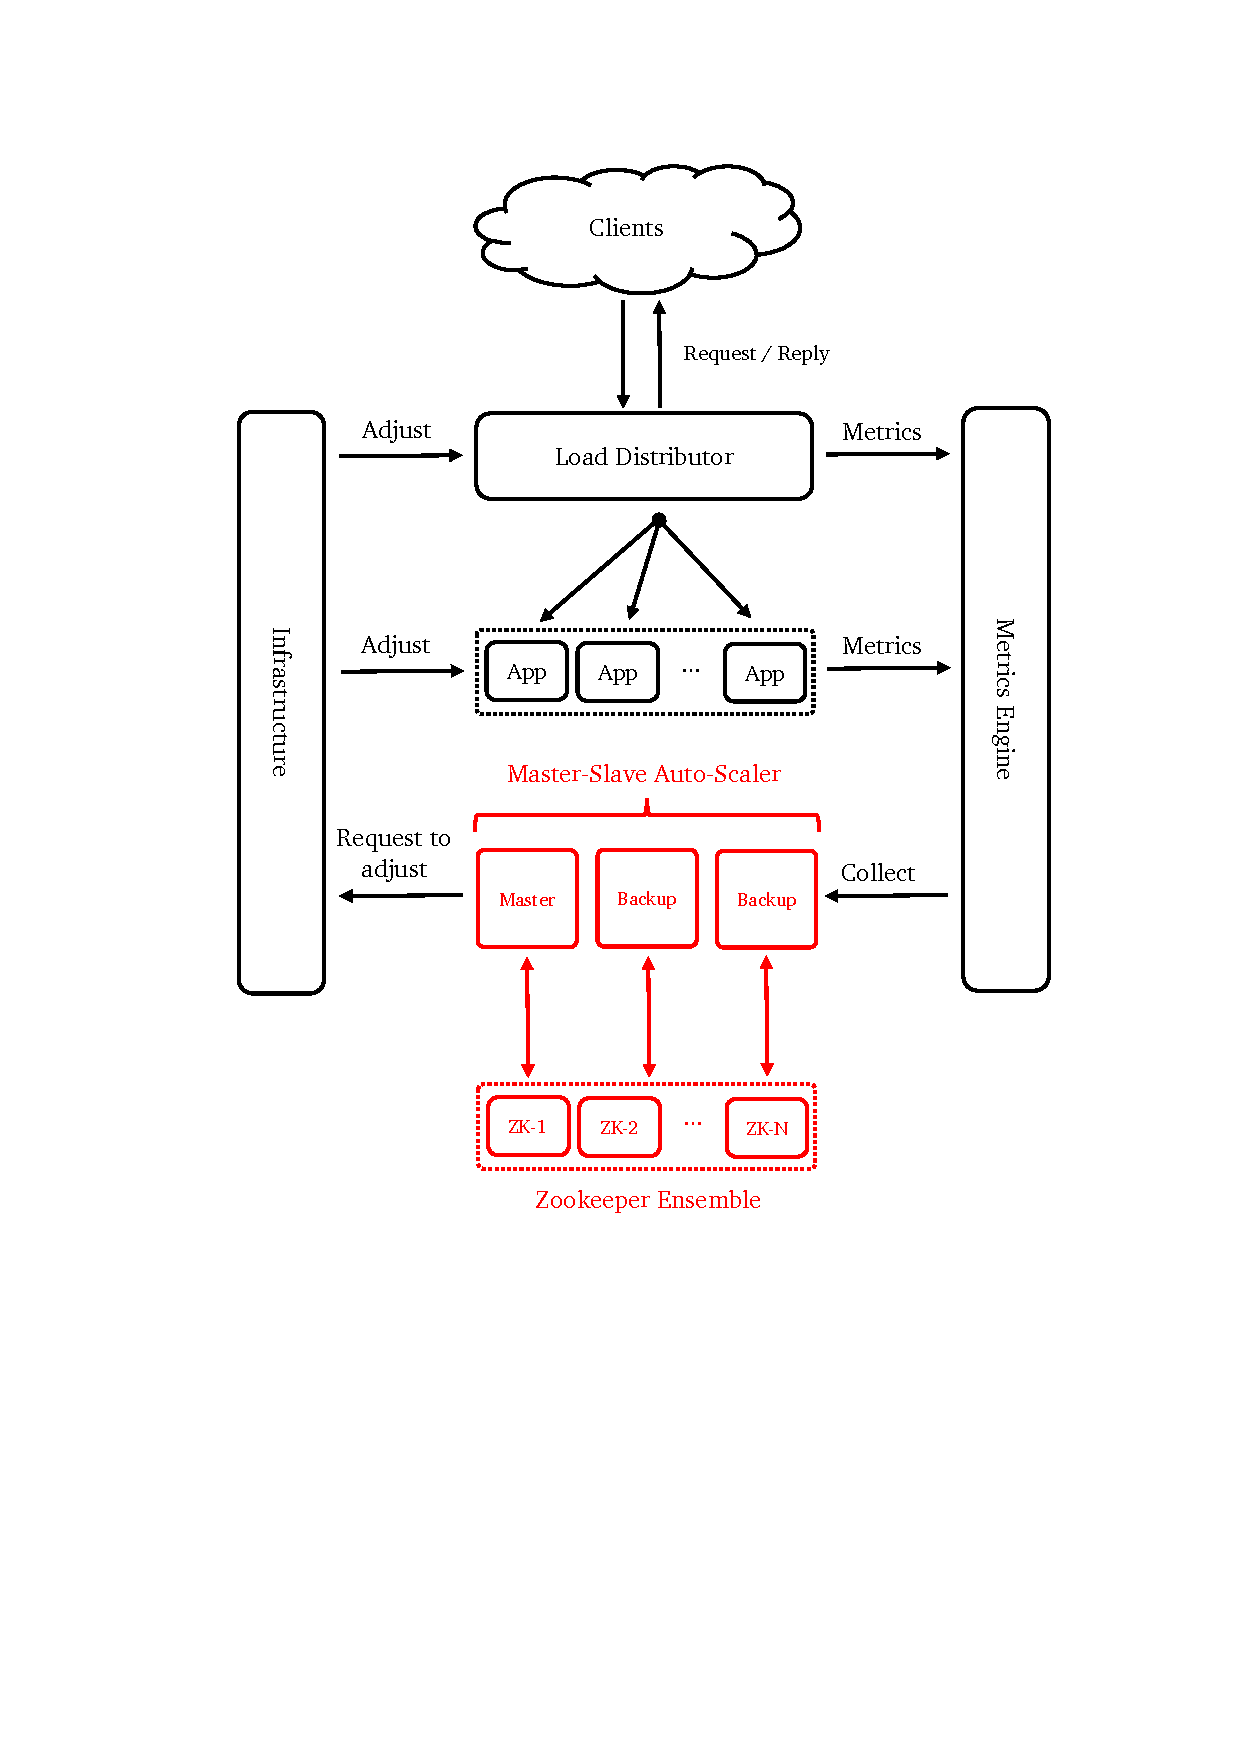
\includegraphics[clip,trim=3cm 9cm 2.5cm 2.5cm]{auto-scaler-master-backup.pdf}
    \centering
    \caption{Architecture of Master-Slave or Global Controller}
    \label{fig:auto-scaler-master-backup}
\end{figure}
\clearpage
\subsubsection{Distributed Without Coordination}
In this architecture, typically Auto-Scaler runs alongside the application instances and each Auto-Scaler instance only \emph{controls} the \emph{local} application. The major difference against global controller is that, in this model each Auto-Scaler makes decision on its own without any form of coordination with other Auto-Scalers. Note that, since each Auto-Scaler instance only controls the local application independent of other application instances, it might lead to sub-optimal decisions because local controllers lack global view of the cluster. Figure~\ref{fig:auto-scaler-dist-wo-coord} illustrates this architecture.
\begin{figure}[!htbp]
    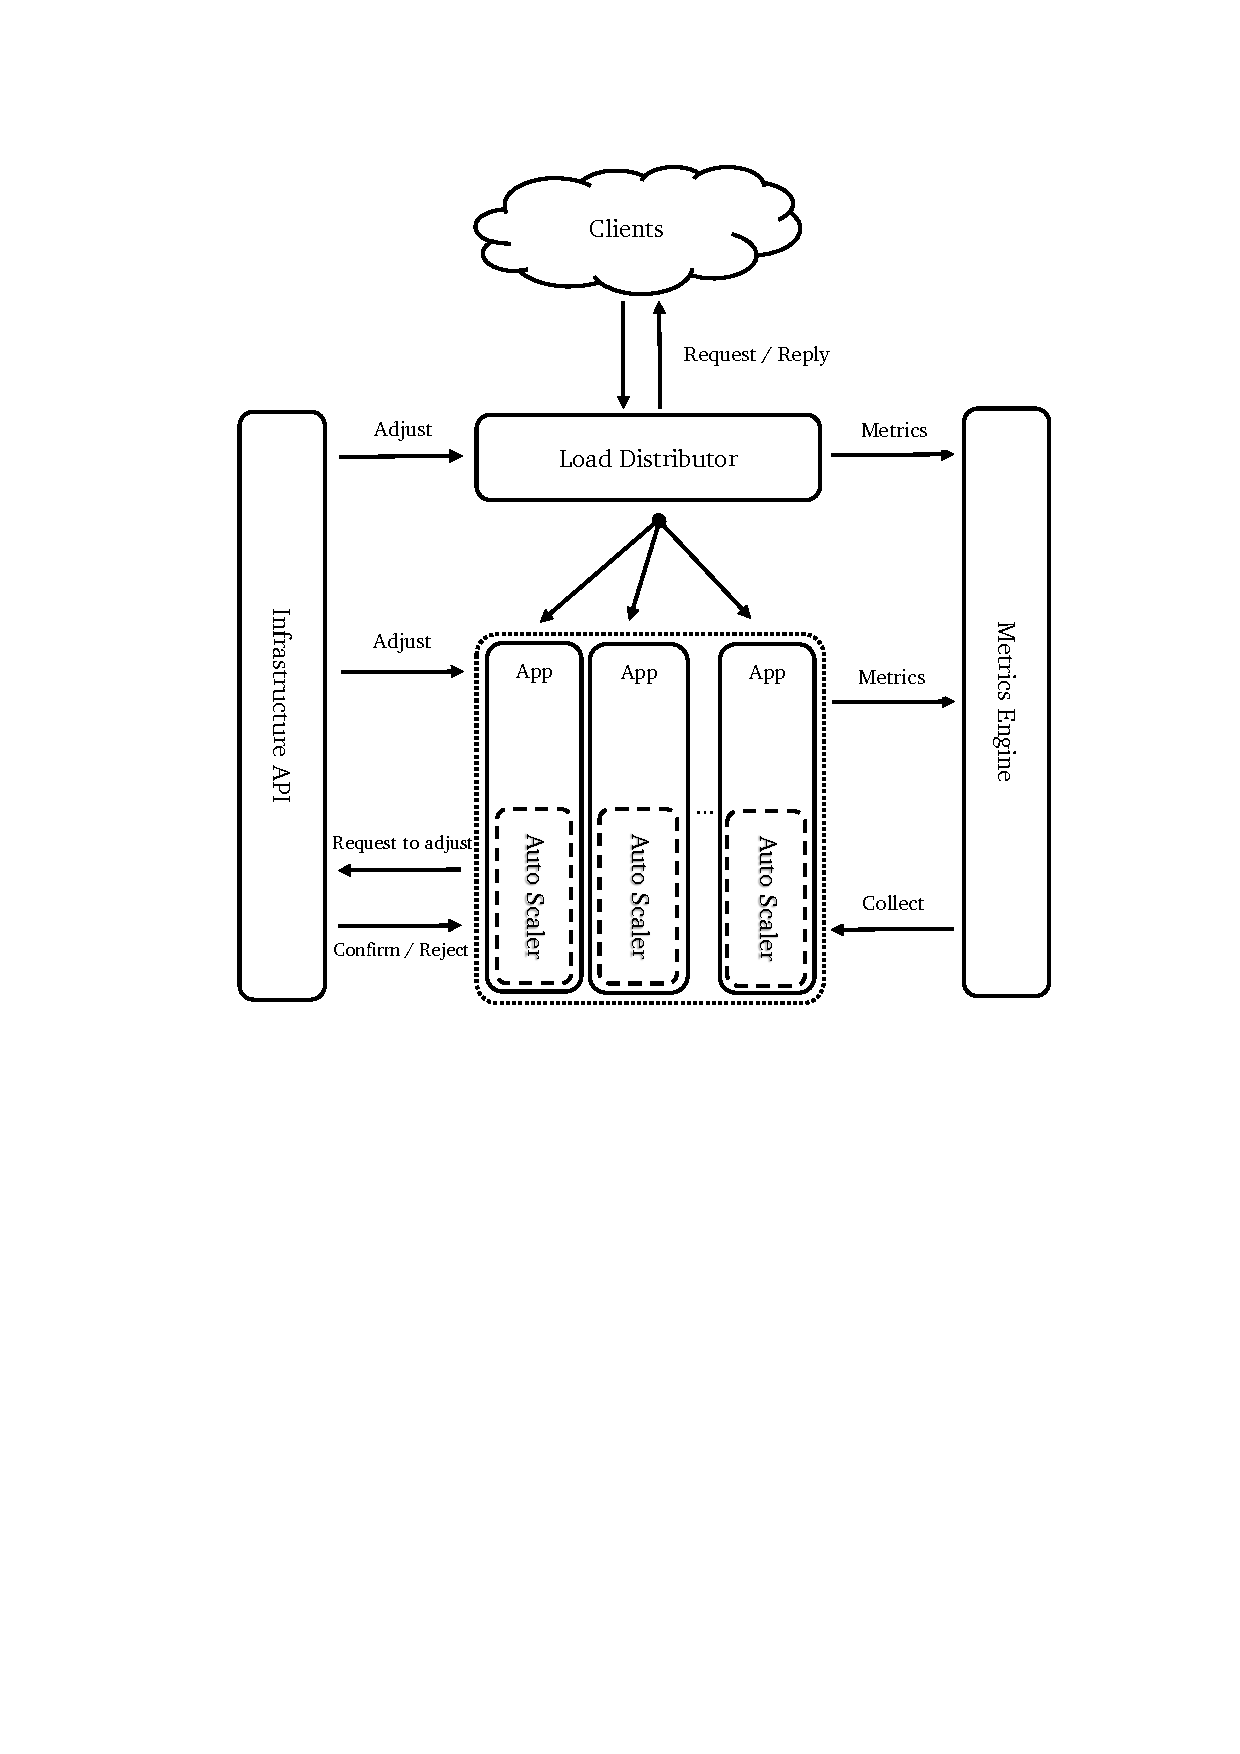
\includegraphics[clip,trim=3cm 12.2cm 2.5cm 2.5cm]{auto-scaler-full-dist.pdf}
    \centering
    \caption{Architecture of Distributed Non-Coordinated Controller}
    \label{fig:auto-scaler-dist-wo-coord}
\end{figure}
\clearpage
\subsubsection{Distributed Coordinated}
This architecture is similar to previous model. However the difference is that, Auto-Scaler components coordinate with each other over a communication channel to gather more information. The amount of communicated information heavily depends on underlying algorithm. In some scenarios only neighbor nodes are contacted. In other cases, all nodes might communicate with each other in order to achieve consensus. Figure~\ref{fig:auto-scaler-dist-coord} depicts this architecture.
\begin{figure}[!htbp]
    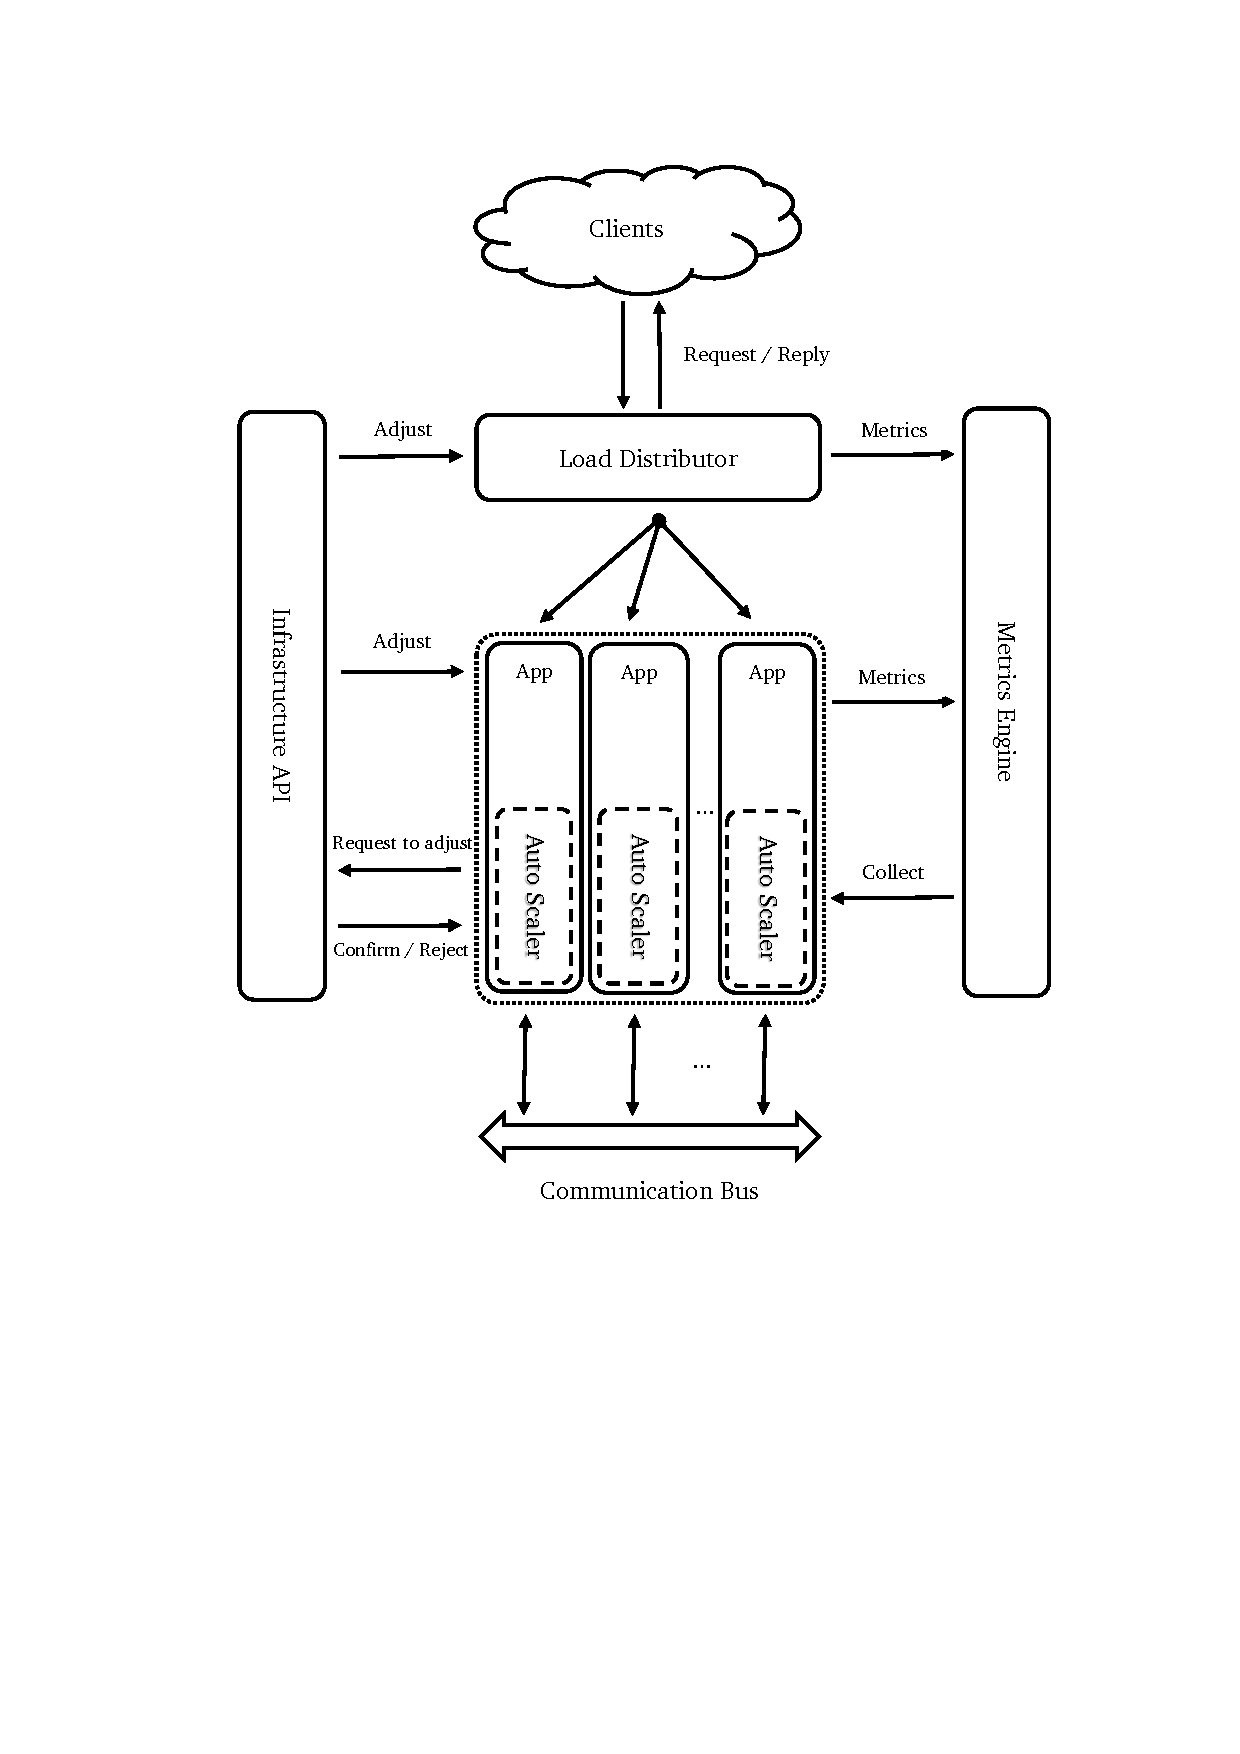
\includegraphics[clip, trim=3cm 9cm 2.5cm 2.5cm]{auto-scaler-dist-coord.pdf}
    \centering
    \caption{Architecture of Distributed Coordinated Controller}
    \label{fig:auto-scaler-dist-coord}
\end{figure}
\clearpage
\subsubsection{Hierarchical Controllers}
This architecture is the mixture of previous models. It's a combination of \emph{Global Controller} and \emph{Distributed Coordinated} model. Local Auto-Scalers communicate with a global controller in order to perform necessary actions. Local Auto-Scalers might also communicate with each other. Additionally, one or more backup controller might also accompany global controller. Furthermore, there might be no limit on who actually performs the actions. Each Auto-Scaler -- whether it is operating in local or global model -- might perform actions independent of the others. Figure~\ref{fig:auto-scaler-hierar} illustrates this architecture.
\begin{figure}[!htbp]
    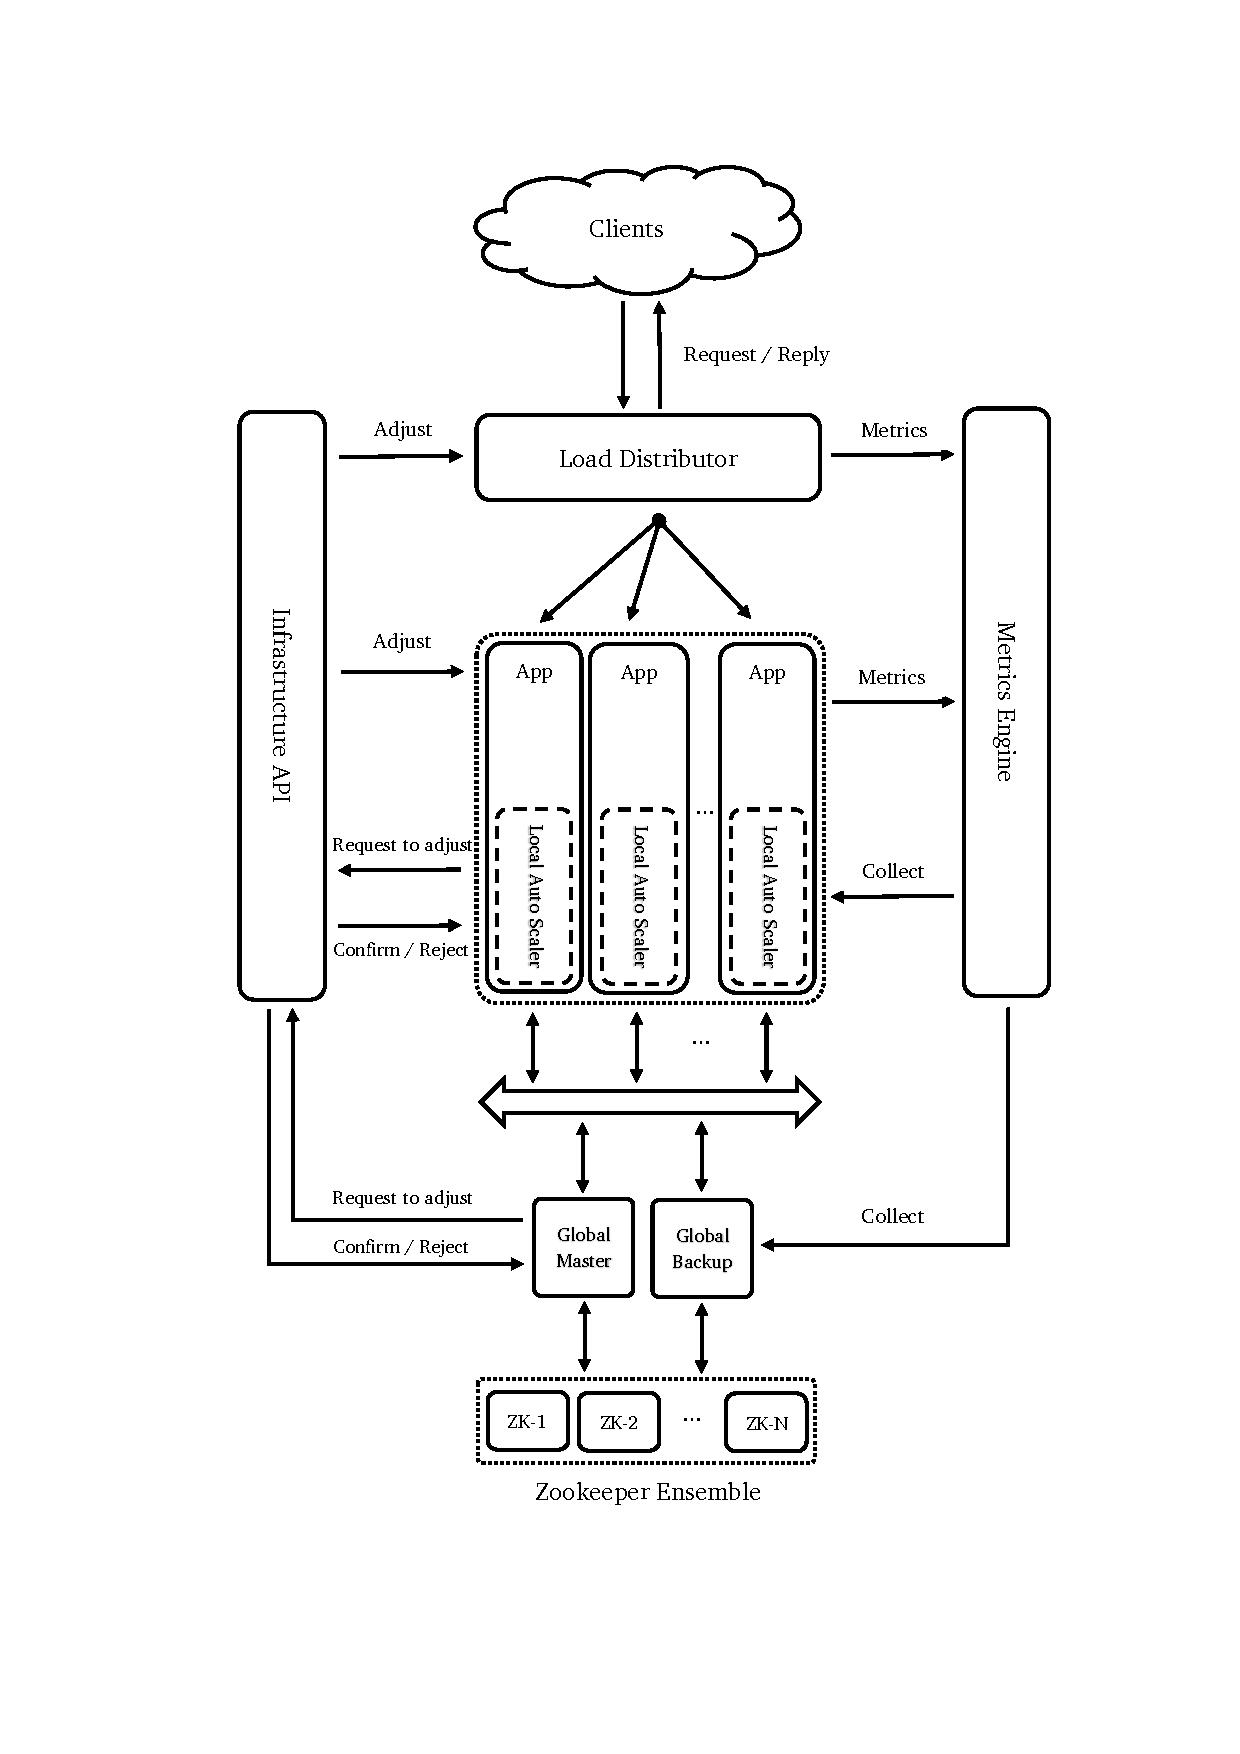
\includegraphics[clip,trim=3cm 4.2cm 2.5cm 2.8cm,scale=0.8]{auto-scaler-hierarchy.pdf}
    \centering
    \caption{Architecture of Hierarchical Controllers}
    \label{fig:auto-scaler-hierar}
\end{figure}
\clearpage
\subsection{Algorithm Family}
\label{ias:alg-fam}

From algorithmic point of view, Auto-Scalers can be classified into 5 different categories.
\begin{itemize}
    \item \textbf{Threshold-Based Policies}
    \item \textbf{Time-Series Analysis}
    \item \textbf{Reinforcement Learning}
    \item \textbf{Queuing Theory}
    \item \textbf{Control Theory}
\end{itemize}
In this section, each category is explained to some extent.
\subsubsection{Threshold-Based Policies} According to Section~\ref{ias:react-proact}, threshold-based approaches follow a purely  reactive approach. It lacks any form of future workload prediction. Threshold-based techniques usually involve a set of constraints which monitors performance data gathered from Metrics Engine. In its naive form, each rule defines an \emph{upper} and/or \emph{lower} bound plus two time periods that define how long that specific metric was above the upper threshold or bellow the lower threshold.

Algorithm~\ref{a:threshold-based} better describes this approach in a pseudocode. Refer to Section~\ref{related} to review list of proposed solutions.
\begin{algorithm}[!htbp]
    \DontPrintSemicolon
    
    \SetKwFunction{LFC}{LoadFromConfig}
    \SetKwFunction{GCMV}{GetCurrentMetricValue}
    \SetKwFunction{AR}{AcquireResource}
    \SetKwFunction{RR}{ReleaseResource}
    \SetKwFunction{DN}{DoNothingDuringGracePeriod}
    
    \SetKwData{ut}{UpperThreshold}
    \SetKwData{up}{UpperPeriod}
    \SetKwData{lt}{LowerThreshold}
    \SetKwData{lp}{LowerPeriod}
    \SetKwData{x}{currentValue}
    \SetKwData{a}{NumberOfResourcesToAcquire}
    \SetKwData{r}{NumberOfResourcesToRelease}
    
    \tcp{upper threshold}
    \ut $\gets$ \LFC{}\;
    \tcp{time period that performance metric was above upper threshold}
    \up $\gets$ \LFC{}\;
    \tcp{lower threshold}
    \lt $\gets$ \LFC{}\;
    \tcp{time period that performance metric was lower than lower threshold}
    \lp $\gets$ \LFC{}\;
    \tcp{number of resources to acquire in each round}
    \a $\gets$ \LFC{}\;
    \tcp{number of resources to release in each round}
    \r $\gets$ \LFC{}\;
    \BlankLine
    \Repeat{\textup{Auto-Scaler is running}} {
        \x $\gets$ \GCMV{}\;
        \BlankLine
        \If{\x > \ut for \up seconds}{
            \tcp{acquire resource}
            \AR{\a}\;
            \DN{}
        }
        \BlankLine
        \If{\x < \lt for \lp seconds}{
            \tcp{release resource}
            \RR{\r}\;
            \DN{}
        }
    }
    \caption{General Work-Flow of Threshold-Based Techniques}
    \label{a:threshold-based}
\end{algorithm}
\subsubsection{Time-Series Analysis} In contrast to threshold-based techniques, time-series analysis approaches are purely proactive or predictive approaches. A \emph{time-series} is a collection of data points sampled and ordered iteratively at uniform time  intervals~\cite{Lorido-Botran2014}. Time-series analysis typically requires to store a history of data points. Hence, storage and computation requirements are more intensive than threshold-based approaches. Refer to Section~\ref{related} for evaluation of prior works in time-series. According to theory of time-series analysis~\cite{TSA}~\cite{Herbst:2013}, time-series can be decomposed into multiple sub components.
\begin{itemize}
    \item \textbf{Season} The season component captures recurring patterns that are composed of one or more frequencies, e.g. daily, weekly or monthly patterns. These dominant frequencies can be determined by using a \emph{Fast Fourier Transformation} (FFT) or by \emph{Auto-Correlation} algorithms.
    \item \textbf{Trend} The trend component can be described by a \emph{monotonically} increasing or decreasing function that can be approximated using common regression techniques.
    \item \textbf{Noise} The noise component is unpredictable outliers of various frequencies with different amplitudes. The noise can be absorbed to some extent by applying smoothing techniques like \emph{Weighted Moving Averages} (WMA), by using \emph{Lower Sampling Frequency} or by a \emph{Low-Pass Filter} that eliminates high frequencies.
\end{itemize}
A time-series has a couple of important characteristics that reveals more information about the values in it. The following represents some of these characteristics.
\begin{itemize}
    \item \textbf{Burstiness} The burstiness defines the impact of fluctuations within the time series and usually calculated by the ratio of the \emph{Maximum Observed Value} to the \emph{Median} within a sliding
    window.
    \item \textbf{Length} The length of the time series mainly influences the accuracy of approximations for the components mentioned above. It can be modeled as \emph{static} or \emph{sliding} window of time.
    \item \textbf{Relative Monotonicity} The relative monotonicity is the maximum number of consecutive monotonic values either \emph{increasing} or \emph{decreasing} within a window and indirectly determines the influence of the noise and seasonal components.
    \item \textbf{Mean, Median, Standard Deviation and Quartiles} These values are important indicators for the distribution of values -- how values are spread -- in time series.
    \item \textbf{Frequency} The frequency of a time series represents the number of values that form a period of interest. This value is an important input as it defines the starting point to find seasonal patterns.
\end{itemize}
\subsubsection{Reinforcement Learning}
Reinforcement Learning is a technique that relies on direct experience from environment. The decision maker -- known as \emph{agent} -- tries to learn the best possible action for each \emph{state} of the environment. The final goal is to maximize the returned \emph{reward}. In the context of Auto-Scaling problem, the agent is the Auto-Scaler component that gets current system state (any group of performance metrics) and tries to minimize/maximize some aspect of the application (response times, throughput, etc.) by performing Scale-In, Scale-Out or No-Action.

In order to formally define Reinforcement Learning environments, some basic terminology~\cite{rlIntro} shall be defined. At each time step $t$, where $t = 0,1,2,\dots$ is a sequence of discrete time steps, the agent receives a representation of the environment's state $s_t \in S$, where $S$ is the set of possible states, and based on that, selects an action, $a_t \in A(s_t)$, where $A(s_t)$ is the
set of possible available actions in state $s_t$. One time step later, as a consequence of performing action $a_t$, the agent receives a numerical reward $r_{t+1}$ and lands in a new state $s_{t+1}$. At each time step, the agent implements a \emph{mapping} from states to probabilities of selecting each possible action. This mapping is called the agent's \emph{policy} and is denoted as $\pi_t$, where $\pi_t(s,a)$ is the probability of taking action $a$ at state $s$ at time $t$. Figure~\ref{fig:rl} depicts this procedure.
\begin{figure}[!htbp]
    \centering
    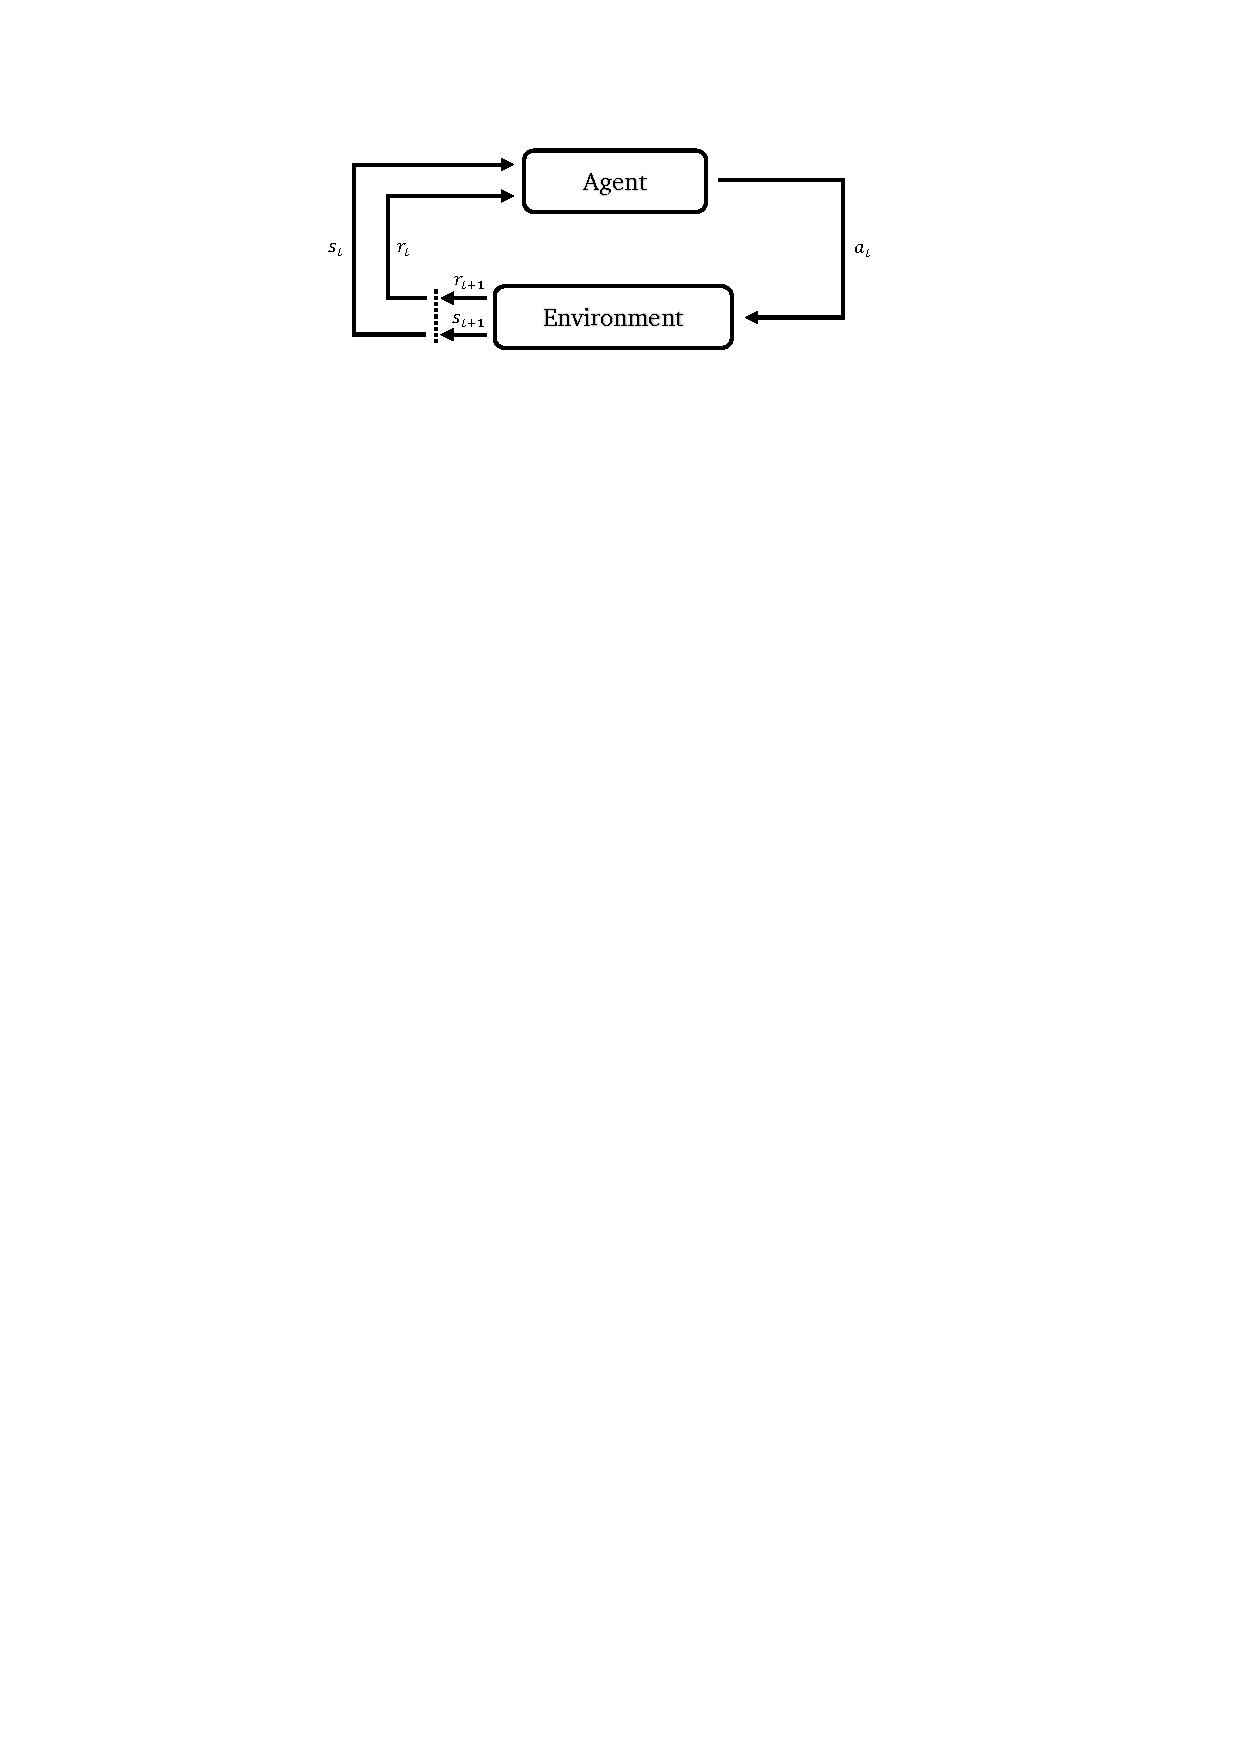
\includegraphics[clip,trim=4cm 23.5cm 4cm 2.5cm]{RL.pdf}
    \caption[Reinforcement Learning Agent]{Reinforcement Learning Agent\footnotemark}
    \label{fig:rl}
\end{figure}
\footnotetext{The figure has been taken from~\textcite{rlIntro}}

In Reinforcement Learning environments future states can be determined only with the current state, regardless of the past history. This is known as \emph{Markov Property}, which formally states that the probability of a moving to a new state $s_{t+1}$ only depends on the current state $s_t$ and action $a$. In other words, it is \emph{independent} of all previous states and actions~\cite{rlIntro}~\cite{Lorido-Botran2014}. Equation~\ref{eq:markov} defines this property.
\begin{equation}
P(s_{t+1} = s',r_{t+1} = r | s_t,a_t) = P(s_{t+1} = s',r_{t+1} = r | s_t,a_t,r_t,s_{t-1},a_{t-1},r_{t-1},\dots,s_1,a_1,r_1,s_0,a_0)
\label{eq:markov}
\end{equation}

A stochastic process that satisfies the Markov property is called a \emph{Markov Decision Process} (MDP). It is typically represented as a 5-tuple consisting of \emph{states}, \emph{actions}, \emph{transitions probabilities}, \emph{reward} and \emph{policy} function.
\begin{itemize}
    \item Set $S$ which represents the state space of the environment.
    \item Set $A$ which represents the total possible actions.
    \item Reward function $R$ defined as $S \times A \rightarrow R$ which represents the reward for each state-action pair. $R(s,a)$ is the reward received after executing action $a$ at state $s$.
    \item Probability distribution $T$ defined as $S \times A \rightarrow P(S)$ which specifies a probability distribution over the set $S$. $P(s'|s,a)$ specifies the probability of landing in state $s'$ assuming that the agent is in state $s$ and performs action $a$.
    \item Policy function $\pi$ defined as $S \rightarrow A$ that maps state $s$ to some action $a$. A policy function that maps state $s$ to \emph{best} possible action -- with highest expected reward -- is called \emph{optimal} policy denoted as $\pi^*$.
\end{itemize}

An important aspect of reward function is that, reward must be accumulated with a \emph{Discount Rate} denoted as $\gamma$. This is introduced to prevent \emph{infinite} reward accumulation and force reward values to converge. Equation~\ref{eq:reward} defines reward function in combination with discount rate.
\begin{equation}
R_t = r_{t+1}+\gamma r_{t+2}+\gamma^2 r_{t+3}+\dots=\sum_{0}^{\infty}\gamma^k r_{t+k+1}
\label{eq:reward}
\end{equation}

Last but not least, under policy $\pi$, \emph{value-state} function $V^\pi(s)$ defines an estimate value of expected reward for state $s$. Equation~\ref{eq:value-state} defines value-state function where $E_\pi$ defines the expected reward value. The value-state function is the core of most Reinforcement Learning techniques. In Section~\ref{design}, two of the techniques used in this thesis will be further discussed. Furthermore, Section~\ref{related} evaluates prior work regarding Reinforcement Learning approaches.
\begin{equation}
V^\pi(s) = E_\pi(R_t|s_t=s)=E_\pi\bigg(\sum_{0}^{\infty}\gamma^k r_{t+k+1}|s_t=s\bigg)
\label{eq:value-state}
\end{equation}
\subsubsection{Queuing Theory}
Queuing theory has been thoroughly used in the context of packet processing to estimate the average wait time until a packet could be routed. The same principle can be applied in the context of Auto-Scaling problem. Clients send requests at a \emph{Mean Arrival Rate} denoted as $\lambda$. Requests are enqueued until they are processed with at a \emph{Mean Service Rate} denoted as $\mu$. Figure~\ref{fig:queue} portrays two architecture of queuing systems. Furthermore, multi-tiered applications are modeled as multiple queues attached \emph{serially} or in \emph{parallel}, depending on the architecture of the application.
\begin{figure}[!htbp]
    \centering
    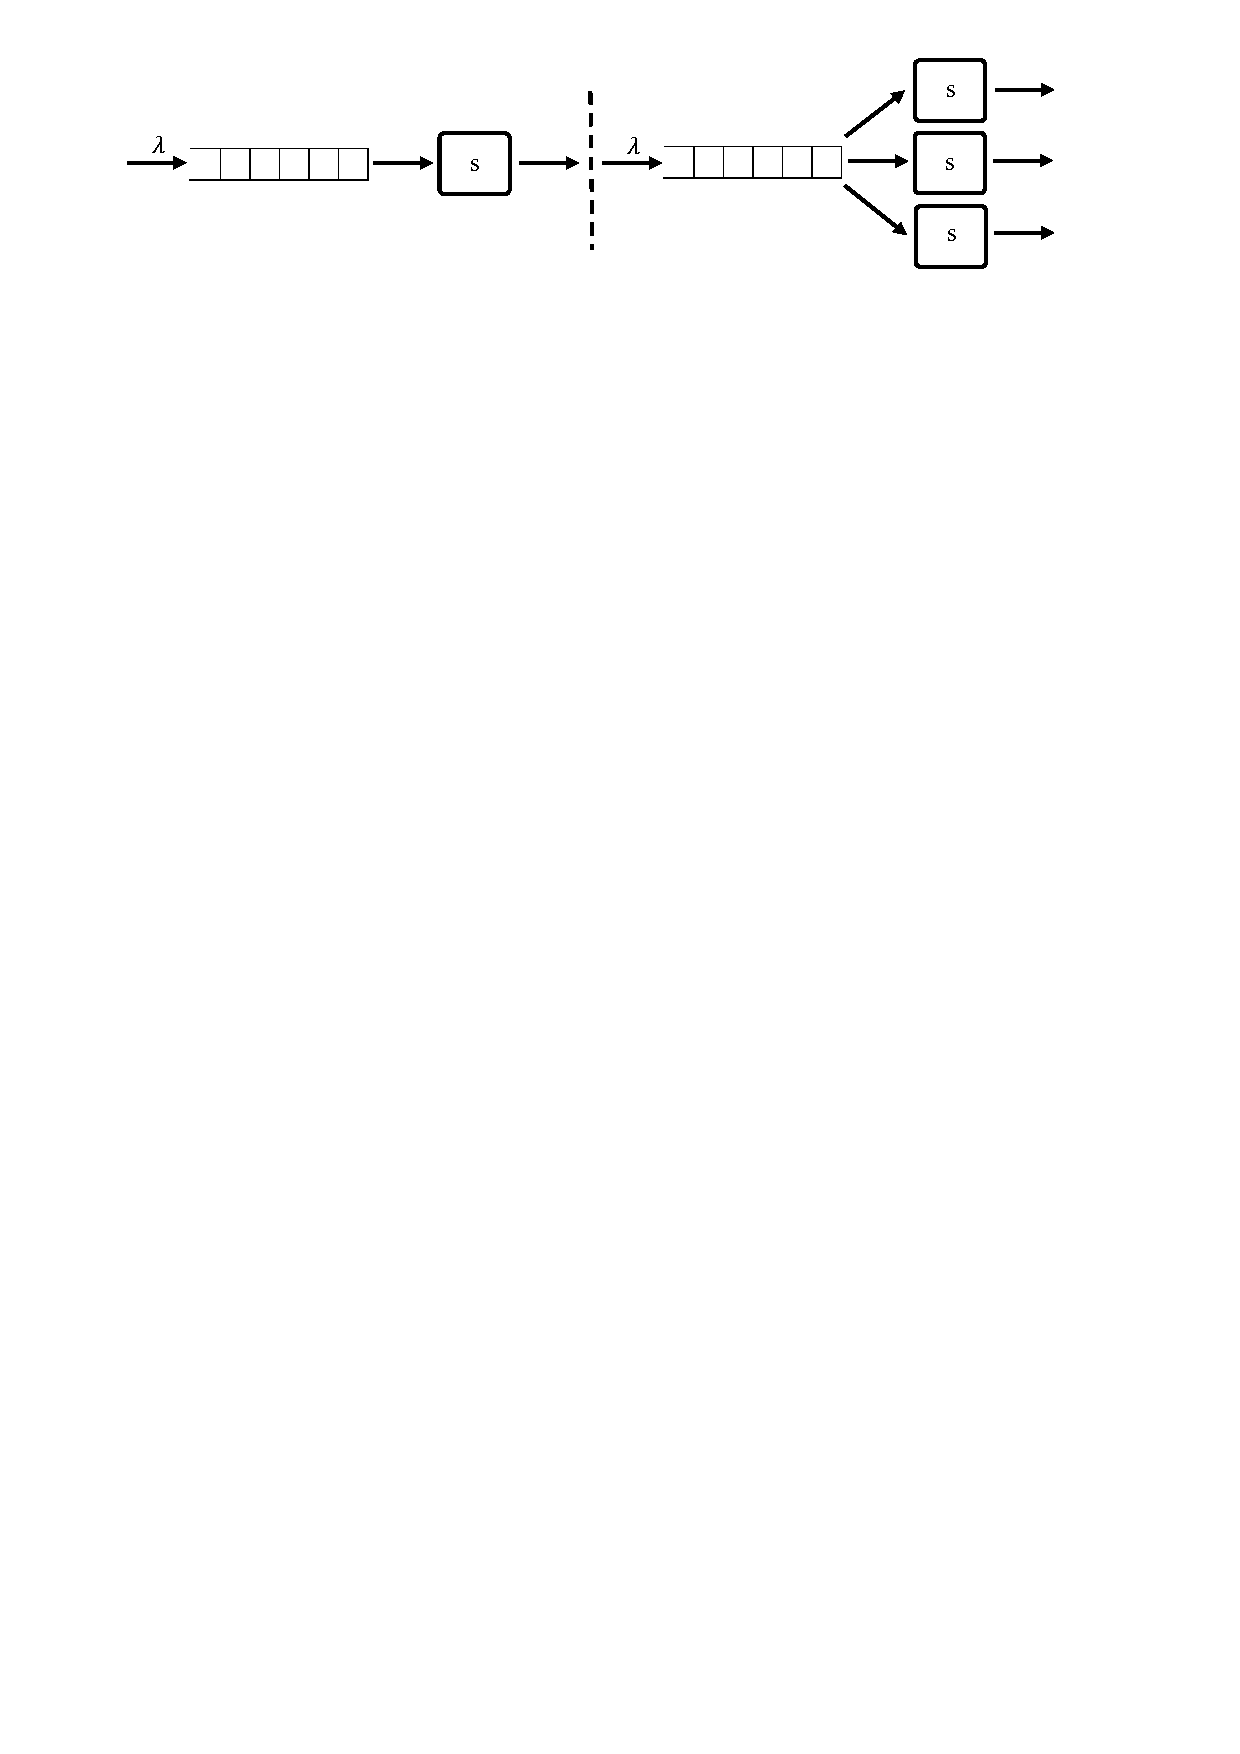
\includegraphics[clip, trim=2cm 25cm 3cm 1cm]{queue.pdf}
    \caption[Queuing Theory]{Queuing Theory with Single Processor (Left), with Multiple Processors (Right)\footnotemark}
    \label{fig:queue}
\end{figure}
\footnotetext{The figure has been taken from~\textcite{Lorido-Botran2014}}

Queuing systems are modeled with \emph{Kendall}'s notation~\cite{kendall1953}. A queue is modeled as $A/B/C/K/N/D$. Each variable is defined and further explained in the following.
\begin{itemize}
    \item \textbf{A} Request inter-arrival time distribution.
    \item \textbf{B} Service time distribution.
    \item \textbf{C} Number of request processors.
    \item \textbf{K} Maximum length of the queue. This is an optional parameter and is set to unlimited if not specified.
    \item \textbf{N} Calling population. This is an optional parameter and is set to unlimited if not specified. This parameter controls the population of requests entering the system. In case of an \emph{open queuing} system, this value is unlimited. While in a \emph{closed queuing} system the population of customers is a finite value.
    \item \textbf{D} Priority order which defines in which order requests will be processed by request processors. This parameter is optional and is set to \emph{First Come First Served} (FCFS) if not specified.
\end{itemize}

Queuing theory is mostly capable of modeling stationary systems with constant parameters defined above. In case of Auto-Scaling problems, these values should be periodically recomputed, since request inter-arrival distribution, service time and number of request processors are changing constantly. These parameters can be re-calculated mostly based on two approaches. First, by applying \emph{analytic} techniques -- suitable for simple queuing systems. Second, by applying \emph{Discrete Event Simulation} (DES) techniques -- suitable for more complex models.
\subsubsection{Control Theory}
Control Theory is categorized as mixture of reactive and proactive systems and decomposed intro three major categories.
\begin{itemize}
    \item \textbf{Open Loop Systems} These systems do not consider any feedback returned by underlying systems. They only consider current state of the system in order to make decision. The output of the system is not considered to check whether it is in stable and desired state.
    \item \textbf{Feedback Systems} These system monitor the output of the system in order to check whether it is complying to defined business conditions. These systems are mainly reactive systems. Figure~\ref{fig:feedback} depicts these controllers.
    \item \textbf{Feed-Forward System} These systems pro-actively try to predict the system's future state and behavior. 
\end{itemize}
\begin{figure}[!htbp]
    \centering
    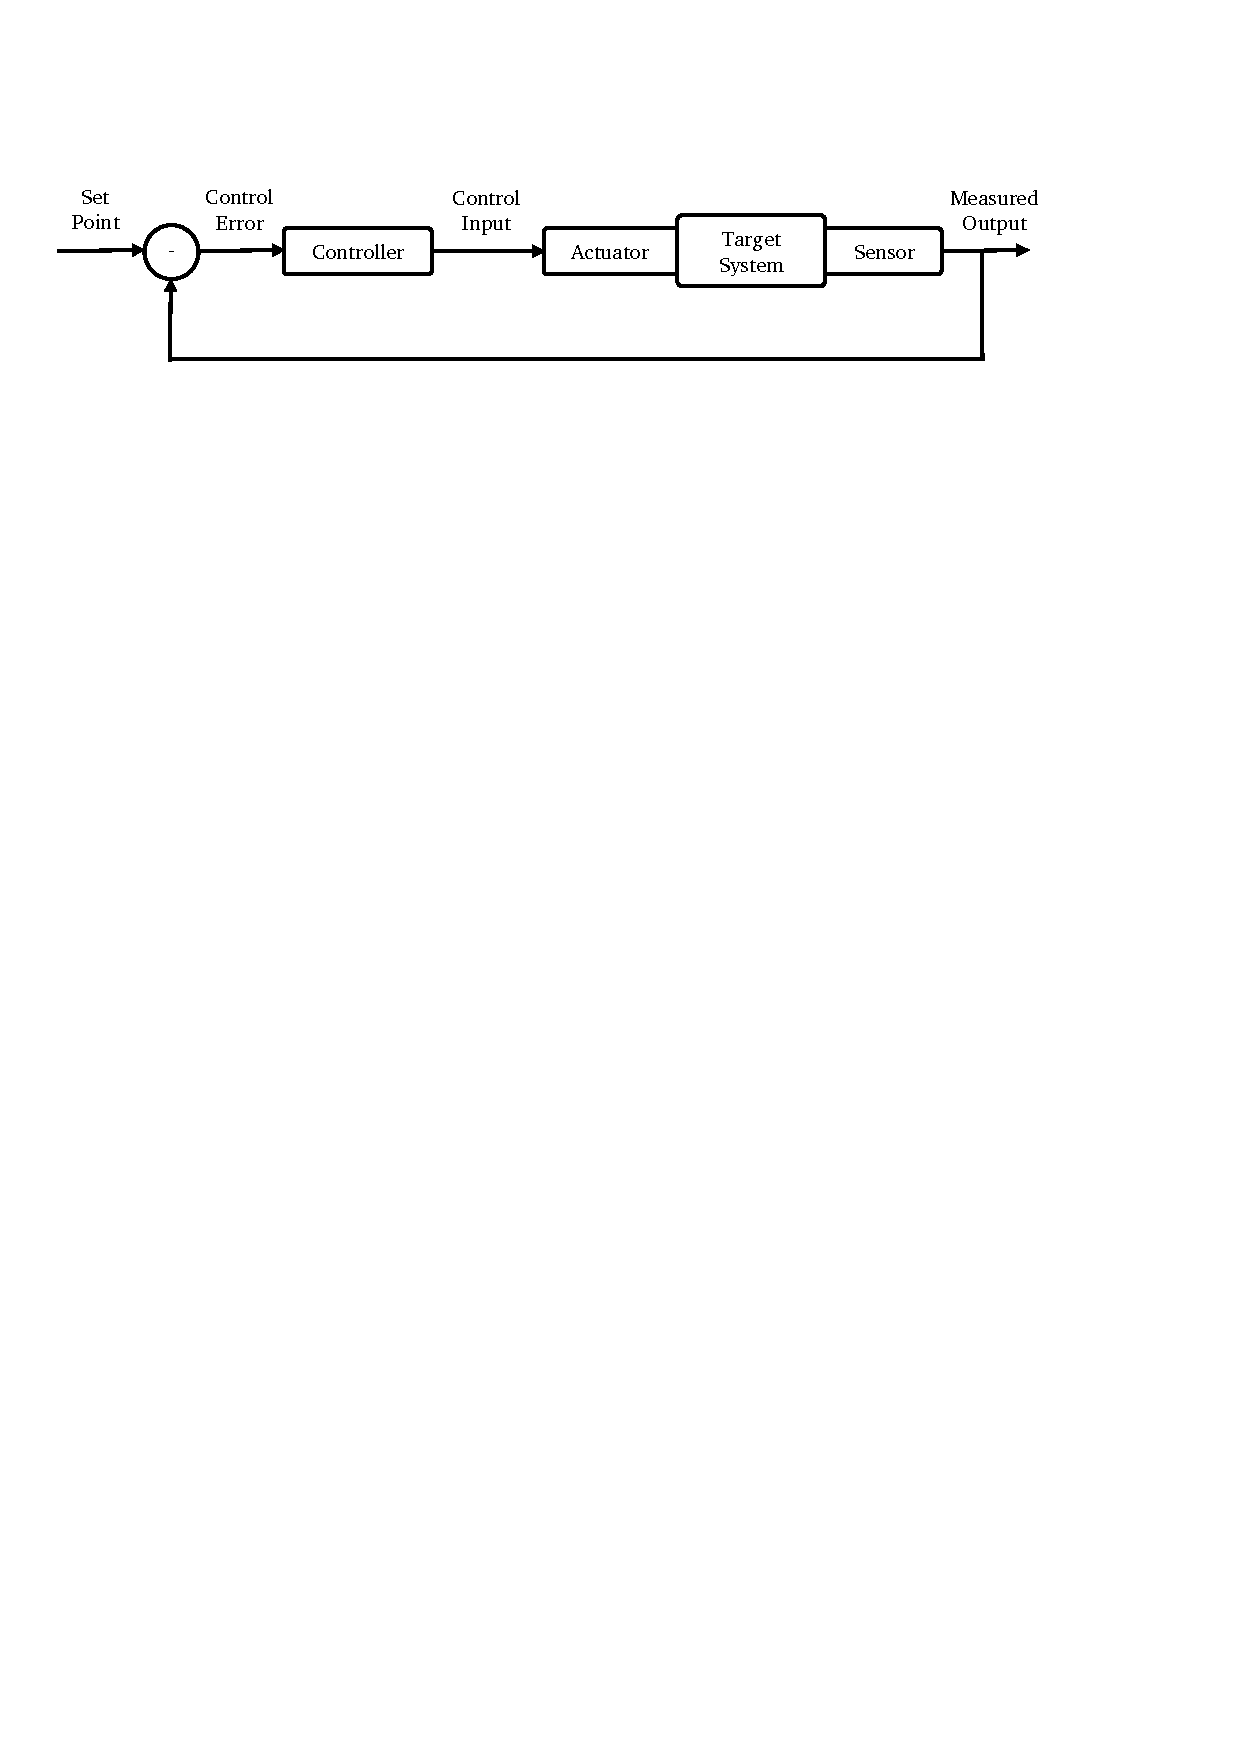
\includegraphics[clip, trim=1.2cm 23.5cm 3.4cm 3cm]{control.pdf}
    \caption[Feedback Control System]{Feedback Control System\footnotemark}
    \label{fig:feedback}
\end{figure}
\footnotetext{The figure has been taken from~\textcite{Patikirikorala:2018}}
Feedback driven control systems are further divided into multiple categories~\cite{Patikirikorala:2018}.
\begin{itemize}
    \item \textbf{Fixed Gain Controllers} The most simple type of feedback control systems. However, the configuration parameters of the controller are fixed during system runtime.
    \item \textbf{Adaptive Controller} These controllers allow to change some of the configuration parameters during runtime which makes them an applicable option for \emph{slowly-changing} environments, but not for suitable for \emph{bursty} workloads.
    \item \textbf{Reconfiguring Controller} In contrast to Adaptive Controllers in which only configuration parameters can be changed at runtime -- controller itself does not change -- in this model the controller itself can also be changed at runtime. With this enhancement, Reconfiguring Controllers are more resilient to bursty workloads.
    \item \textbf{Model Predictive Controller} These controllers mix some \emph{predicative} features into feedback controllers which make them even more resilient to unanticipated workloads.
\end{itemize}
\section{Conclusion}
\label{ias:conc}

In this chapter, different architectural aspects and major design considerations of Auto-Scalers have been discussed. As mentioned, it is a multi-dimensional space of features and capabilities. Many of the current proposals do not map to one category, but combine divergent set of features. Section~\ref{related} compares and evaluates prior research on different systems.